\documentclass{beamer}

\usepackage{amssymb}
\usepackage{latexsym}
\usepackage{amsmath}
\usepackage{amsfonts}
\usepackage{graphicx}
\usepackage{color} %% to use color: \textcolor{color}{words to be in color} 
\usepackage{tikz}


\usepackage[T1]{fontenc}
\usepackage[condensed,math]{anttor}
\usepackage[english]{babel}
\usepackage[latin1]{inputenc}


% font definitions, try \usepackage{ae} instead of the following
% three lines if you don't like this look
\usepackage{mathptmx}
\usepackage[scaled=.90]{helvet}
\usepackage{courier}



\mode<presentation>{
\usetheme{CambridgeUS}
\usecolortheme{dolphin}

\setbeamercovered{transparent}
%gets rid of bottom navigation bars
\setbeamertemplate{footline}[page number]{}
%gets rid of navigation symbols
\setbeamertemplate{navigation symbols}{}
}


\newcommand{\A}{\mathcal A}
\newcommand{\AAA}{\mathfrak A}
\newcommand{\B}{\mathcal B}
\newcommand{\BBB}{\mathfrak B}
\newcommand{\CCC}{\mathcal C}
\newcommand{\DDD}{\mathcal D}
\newcommand{\F}{\mathcal F}
\newcommand{\G}{\mathcal G}
\newcommand{\HHH}{\mathcal H} %for Hilbert space
\newcommand{\III}{\mathcal I}
\newcommand{\LLL}{\mathcal L} % for lattice
\newcommand{\PPP}{\mathcal P}
\newcommand{\QQQ}{\mathcal Q}
\newcommand{\M}{\mathcal M}
\newcommand{\MMM}{\mathfrak M}
\newcommand{\NNN}{\mathcal N} %for nest
\newcommand{\RRR}{\mathcal R}
\newcommand{\SSS}{\mathcal S}
\newcommand{\W}{\mathcal W}
\newcommand{\ZZZ}{\mathcal Z}
\newcommand{\supp}{\mathop{\mathrm supp}}
\newcommand{\TT}{\mathcal T}
\newcommand{\II}{\mathrm{II}}

\newcommand{\Lat}{\mathrm{Lat}}
\newcommand{\Alg}{\mathrm{Alg}}
\newcommand{\tensor}{\mathop{\bar \otimes}}
\newcommand{\tr}{\tau}
\newcommand{\Var}{\mathrm Var}
\newcommand{\Naf}{\mathrm Naf}


\newcommand{\C}{\mathbb C }
\newcommand{\R}{\mathbb R}
\newcommand{\Z}{\mathbb Z}
\newcommand{\N}{\mathbb N}


\title{On a new class of non selfadjoint algebras }

%\subtitle{}

% - Use the \inst{?} command only if the authors have different
%   affiliation.
%\author{F.~Author\inst{1} \and S.~Another\inst{2}}
\author{Yuan Wei \inst{AMSS}}

% - Use the \inst command only if there are several affiliations.
% - Keep it simple, no one is interested in your street address.
\institute[Academy of Mathematics and Systems Science, Chinese Academy of
Sciences] { \inst{1}%
Institute of Mathematics}

\date{\today (Chongqing University)}


% This is only inserted into the PDF information catalog. Can be left
% out.
\subject{Talks}


\pgfdeclareimage[height=.5 cm]{university-logo}{amss-logo.png}
\logo{\pgfuseimage{university-logo}}




% If you wish to uncover everything in a step-wise fashion, uncomment
% the following command:

%\beamerdefaultoverlayspecification{<+->}

\begin{document}

\begin{frame}
\titlepage
\end{frame}


\begin{frame}
\frametitle{Notations}

\begin{itemize}
  \item $\C$: the field of complex numbers;\vspace{.3cm}
  \pause
  \item $\HHH$: a separable Hilbert spaces, e.g. $l^2(\Z)$,
  $l^2(\Z_{n})$\vspace{.3cm}
  \pause
  \item $\B(\HHH)$: the algebra of all bounded linear
        operators on $\HHH$, e.g. $M_n(\C)$
\end{itemize}
\end{frame}

\begin{frame}
\frametitle{The Legacy of John Von Neumann}
\begin{center}
\includegraphics[scale = 0.4]{VNC.jpg}
\end{center}
\end{frame}

\begin{frame}
\begin{theorem}[Von Neumann double commutant theorem(1929) \\ 
\qquad \qquad $\mbox{Zur Algebra der Funktionaloperatoren}$]
%Algebra of the function operator
A self adjoint subalgebra $\AAA$ of $\B(\HHH)$ is a 
von Neumann algebra if and only if $\AAA'' = \AAA$.
\end{theorem}


Examples:\\
\begin{center}
\begin{tabular}{ccc}
   \visible<2->{$M_n(\C)$}&\visible<2->{\Leftrightarrow}
    &\visible<2->{$\B(\HHH)$} \\
   \visible<3->{Finite dimensional} & & 
    \visible<3->{Infinite dimensional} \\
   \visible<4->{has trace} &  & \visible<4->{does not have trace}
\end{tabular}
\end{center}

\vspace{1cm}

\visible<5->{\bf{Is there an infinite dimensional "finite" factor?}}
\end{frame}

\begin{frame}
\frametitle{1934, Murray}
\begin{theorem}
If $\AAA$ is a factor and $E_1 \in \AAA$ and $E_2 \in \AAA'$, then $E_1 E_2
\neq 0$ if $E_1$, $E_2 \neq 0$.
\end{theorem}

\only<2>{
\begin{figure} [H]
     \centering
      \includegraphics[scale=.5]{fig1.png}
     \caption{$l^{2}(\Z_4) \otimes l^{2}(\Z_5), \qquad \AAA \cong M_{4}(\C),
     \quad \AAA' \cong M_5{\C}$}
\end{figure}
}

\only<3>{
\begin{figure} [H]
     \centering
      \includegraphics[scale=.5]{fig2.png}
     \caption{$l^{2}(\Z_4) \otimes l^{2}(\Z_4) \oplus l^{2}(\Z_3) \otimes
     l^{2}(\Z_3) \oplus l^{2}(\Z_5) \otimes l^{2}(\Z_3)$}
\end{figure}
}


\end{frame}

\begin{frame}
\frametitle{Bernstein's Theorem's analogy}

\begin{tabular}{ccc}
Ranges of projections & & Cardinal numbers of sets \\
&\Leftrightarrow & \\
Partial isometries &  & one-to-one correspondence
\end{tabular}

\visible<2->
{\begin{theorem}
If $E$ and $F$ are projections in a von Neumann algebra $\AAA$ such that
$E \preceq F$ and $F \preceq E$, then $E\sim F$.
\end{theorem}
}
\end{frame}

\begin{frame}
\begin{center}
\begin{tabular}{cc}
Factor Type  &  Range of the dimension function \\
\visible<1->{I$_n (n < \infty)$} & \visible<1->{$\{0, \frac{1}{n}, \frac{2}{n},
\ldots, \frac{n}{n} \}$} \\ 
\visible<2->{I$_{\infty}$}  & \visible<2->{$\{0, 1, 2, \ldots, \infty \}$}\\
\visible<3->{II$_{1}$} & \visible<3->{$[0, 1]$}\\
\visible<4->{II$_{\infty}$} & \visible<4->{$[0, \infty]$}\\
\visible<5->{III} & \visible<5->{$\{0, \infty \}$}
\end{tabular}
\end{center}

\vspace{1cm}

\visible<6->{\bf{The immediate problem: \\
obtain an example of a case other than type I.}}
\end{frame}

\begin{frame}
\frametitle{Exmaple of II$_1$ factors:}

\begin{center}
\includegraphics[scale = 0.35]{fig3.png}\\
\caption{\small{$\alpha$ is a binary number}}
%$y = x + \alpha mod 1$ with linear Lebesgue measure 
\end{center}

\begin{center}
\visible<2->{
\begin{tabular}{cc}
$\AAA$  &  $\AAA'$\\
$M_x: (M_xf)(x,y) = xf(x,y)$ & $M_y: (M_yf)(x,y) = yf(x,y)$ \\
$L_{\alpha}: (L_{\alpha}f)(x,y) = f(x + \alpha, y)$ & $R_{\alpha}:
(R_{\alpha}f)(x,y) = f(x , y + \alpha)$
\end{tabular}
}

\vspace{.5cm}

\visible<3->{$Tr_{\AAA}(A) = \langle A\xi, \xi \rangle$, \qquad $\xi(x,y) =
\delta(x,y)$.}
\end{center}
\end{frame}

\begin{frame}
\begin{align*}
Tr_{\AAA}(M_x L_{\alpha}) &= \sum_{\beta}\int x \delta(x+\alpha, x+ \beta)
\delta(x, x+ \beta) dx \\
& = \int x \delta(x+\alpha, x) dx = 0 = Tr_{\AAA}(L_{\alpha}M_{x})
\end{align*}
\end{frame}

\begin{frame}
\frametitle{Group factors}
 
$G: $ a discrete group, e.g. $\Pi = \cup_{n}S_{n}$.\\

$l^{2}(G) = \{\sum_{g \in G} a_g e_{g} | \sum_{g \in G} |a_g|^2 < \infty \}$

\vspace{1cm}

\visible<2->{
\begin{tabular}{cc}
Left regular representation & Right regular representation\\
$\AAA = \{L_h | h \in G \}'' $ & $\AAA' = \{R_h | h \in G \}''$\\
$L_{h}(\sum_{g \in G} a_g e_{g} ) = \sum_{g \in G} a_g e_{hg} $ &
$R_{h}(\sum_{g \in G} a_g e_{g} ) = \sum_{g \in G} a_g e_{hg^{-1}} $ 
\end{tabular}
}

\vspace{.5cm}
\begin{center}
\visible<3->{$Tr_{\AAA}(A) = \langle Ae_g, e_g \rangle$.}
\end{center}
\end{frame}

\begin{frame}
$\Pi$ is a infinite-conjugacy-class group.
\begin{proof}
\visible<2->{Suppose $g \in S_n$ and $g(i) = j$, $i,j \leq n$.}\\
\visible<3->{Let $g_m = (j,n+m)$, $m = 1, 2, \ldots$.}\\
\visible<4->{Thus $g_m g g_m^{-1}(n+m) = i$ and $\{g_m g g_m^{-1} | m = 1, 2
\ldots\}$ is an infinite set of conjugates of $g$. }
\end{proof}

\visible<5->{
Fact:\\
Suppose $\AAA$ is a type II$_1$ factor, then for any $n > 0$, there is a 
subalgebra $\MMM$ of $\AAA$ such that $\MMM \cong M_n(\C)$.
}


\end{frame}

\begin{frame}
\begin{definition}[Hyperfinite II$_1$ factor]
The hyperfinite II$_1$ factor $R$ is a countably generated factor of type II$_1$
such that $\forall \varepsilon > 0$ and $\{A_1, \ldots, A_n \} \subset
(R)_1$(unit ball of $R$), there is a finite type I subfactor $\NNN$ of $R$ and 
$\{B_1, \ldots, B_n \} \subset (\NNN)_1$ such that $\| A_i - B_i \|_2 <
\varepsilon$ when $i \in \{1, \ldots, n \}$.
\end{definition}

\visible<2->{
\begin{theorem}
\bf{$L_{\Pi}$ is the only hyperfinite II$_1$ factor.}
\end{theorem}
}
\end{frame}



\begin{frame}
\frametitle{Constructions of hyperfinie II$_1$ factor}
\begin{itemize}
  \item For any amenable i.c.c group $G$, $L_G \cong R$;\vspace{.3cm}
  \pause
  \item $R \cong M_{n_1}(\C) \bar{\otimes} M_{n_2}(\C) \bar{\otimes} M_{n_3}(\C)
  \bar{\otimes} \cdots$
\end{itemize}

\visible<3->{
$M_{n_1}(\C) \otimes I \subset M_{n_1}(\C) \otimes M_{n_2}(\C) \otimes I \subset
M_{n_1}(\C) \otimes M_{n_2}(\C) \otimes M_{n_3} \otimes I \subset \cdots$\\
The ascending family of finite dimensional algebras is dense in $R$. 
}

\begin{center}
 \only<4>{
 $M_2(\C) \otimes I '$ = \left( {\begin{array}{cc}
 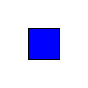
\begin{tikzpicture}
\draw[fill=blue] (0,0) rectangle (0.4,0.4);
\end{tikzpicture} &  \\
  & 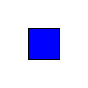
\begin{tikzpicture}
\draw[fill=blue] (0,0) rectangle (0.4,0.4);
\end{tikzpicture}  \\
 \end{array} } \right)
 }
 
 \only<5>{
  $M_2(\C) \otimes I '$ = \left( {\begin{array}{cccc}
 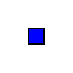
\begin{tikzpicture}
\draw[fill=blue] (0,0) rectangle (0.2,0.2);
\end{tikzpicture} &  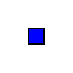
\begin{tikzpicture}
\draw[fill=blue] (0,0) rectangle (0.2,0.2);
\end{tikzpicture}  & &\\
  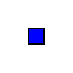
\begin{tikzpicture}
\draw[fill=blue] (0,0) rectangle (0.2,0.2);
\end{tikzpicture} & 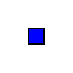
\begin{tikzpicture}
\draw[fill=blue] (0,0) rectangle (0.2,0.2);
\end{tikzpicture}  & &\\
& & 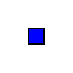
\begin{tikzpicture}
\draw[fill=blue] (0,0) rectangle (0.2,0.2);
\end{tikzpicture} &  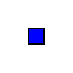
\begin{tikzpicture}
\draw[fill=blue] (0,0) rectangle (0.2,0.2);
\end{tikzpicture} \\
& & 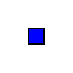
\begin{tikzpicture}
\draw[fill=blue] (0,0) rectangle (0.2,0.2);
\end{tikzpicture} & 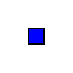
\begin{tikzpicture}
\draw[fill=blue] (0,0) rectangle (0.2,0.2);
\end{tikzpicture}
 \end{array} } \right)
 }
 
 \only<6>{
 $ M_2(\C) \otimes M_2(\C) \otimes I '$ =\left( {\begin{array}{cccc}
 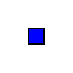
\begin{tikzpicture}
\draw[fill=blue] (0,0) rectangle (0.2,0.2);
\end{tikzpicture} &  & &\\
  & 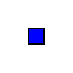
\begin{tikzpicture}
\draw[fill=blue] (0,0) rectangle (0.2,0.2);
\end{tikzpicture}  & &\\
& & 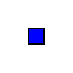
\begin{tikzpicture}
\draw[fill=blue] (0,0) rectangle (0.2,0.2);
\end{tikzpicture} & \\
& & & 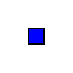
\begin{tikzpicture}
\draw[fill=blue] (0,0) rectangle (0.2,0.2);
\end{tikzpicture}
 \end{array} } \right)
 }
 
 \end{center}
\end{frame}

\begin{frame}
\begin{tabular}{ccc}
$M_{n_1}(\C) \otimes M_{n_2}(\C) \otimes \cdots \otimes M_{n_k}(\C) \otimes
\cdots$ & \Leftrightarrow & $\Pi_{p} p^{a_{p}}$
\end{tabular}

\vspace{.3cm}

$a_{p} = \sum_{k} b_{p}^{k}$, $n_{k} = \Pi_{p} p^{b^{k}_{p}}$

\vspace{.3cm}

\visible<2->{
\begin{tabular}{ccc}
$\AAA_1 = M_{n_1}(\C) \otimes M_{n_2}(\C) \otimes \cdots \otimes M_{n_k}(\C)
\otimes \cdots$ & \Leftrightarrow & $\Pi_{p} p^{a_{p}}$ \\
$\AAA_2 = M_{m_1}(\C) \otimes M_{m_2}(\C) \otimes \cdots \otimes M_{m_k}(\C)
\otimes \cdots$ & \Leftrightarrow & $\Pi_{p} p^{b_{p}}$
\end{tabular}

\begin{theorem}[J. Glimm]
The $C^{*}$ algebras $A_1$ and $A_2$ are isomor\alphac if and only if $\Pi_{p}
p^{a_{p}} = \Pi_{p} p^{b_{p}}$.
\end{theorem}
}
\end{frame}

\begin{frame}
\frametitle{Some results about hyperfinite factor of type II$_1$}
\begin{columns}
\column{.4\textwidth}
Alain Connes (1976) 
\column{.4\textwidth}
V. Jones (1983)
\end{columns}

\begin{columns}
\column{.4\textwidth}
All subfactors of $R$ are isomor\alphac to $R$ or finite dimensional.
\column{.4\textwidth}
The possible values of the index for subfactors of $R$:
\begin{align*}
&\{4\cos^{2}(\frac{\pi}{n}) | n = 3, 4, \ldots \} \\
&\cup \{r \in \R | r \geq 4 \}
\cup \{\infty \}
\end{align*}
\end{columns}

\end{frame}

\begin{frame}
\frametitle{Non-selfadjoint algebras}

\begin{definition}[Kadison, Singer (1960)]
If $\MMM$ is a factor and $\AAA$ a maximal abelian (selfadjoint) subalgebra of
$\MMM$, a subalgebra $\mathcal{T}$ of $\MMM$ will be said to be ``triangular
in $\MMM$ with diagonal $\AAA$ when $\mathcal{T} \cap \mathcal{T}^{*} = \AAA$.
\end{definition}

\visible<2->{
\begin{theorem}
If $\AAA$ is a maximal triangular algebra on a finite dimensional space,
then there is an orthonormal basis such that $\AAA$ is the algebra of all 
operators with upper triangular matrices relative to this basis.
\end{theorem}
}
\end{frame}

\begin{frame}
\frametitle{Some Problems}

{\bf Operator Theory:} Invariant Subspace Problem asks whether every
bounded operator on a (separable) Hilbert space has a (nontrivial)
invariant subspace.\\

\vspace{.2cm}

\visible<2->{{\bf Algebraic Version:} Whether every abelian subalgebra of B(H)
has a (common) invariant subspace.}\\

\vspace{.2cm}

\visible<3->{{\bf Kadison's Transitive Algebra Problem:} If A is a transitive
algebra on H (or A has no nontrivial invariant subspace), then is the
weak-operator closure of A equals to B(H)?}

\vspace{.2cm}

\visible<4->{{\bf The invariant subspace problem relative to a factor:}
If every operator in the factor $\AAA$ has a non-trivial invariant subspace 
affiliated with $\AAA$.

}

\end{frame}

\begin{frame}
\frametitle{Some Results}

{\bf Enflo(1976):} There exists a Banach space and a bounded linear
operator on it without any non-trivial invariant subspace. \\

\vspace{.3cm}

\visible<2->{
{\bf Arveson(1967) :} If $\AAA$ is a transitive operator algebra,
and if $\AAA$ contains a m.a.s.a, then $\AAA = \B(\HHH)$.\\
}

\vspace{.3cm}

\visible<3->{
{\bf Haagerup and H. Schultz(2006):} If $T$ in a II$_1$ factor $\AAA$ has
a non-Dirac Brown measure, then T has a non-trivial hyperinvariant subspace.

\begin{align*}
d_{\mu_T}(x + iy) = \frac{1}{2\pi}\nabla^2 log\Delta[T - (x+iy)I]dxdy, 
\Delta(T) = exp{\tau(log|T|)}. 
\end{align*}

if $T \in M_n(\C)$, $\Delta(T) = |detT|^{\frac{1}{n}}$ and $\mu_T = 
\frac{1}{n} \sum^{n}_{i=1} \delta_{\lambda_i}$.
}

\end{frame}


\begin{frame}

\begin{itemize}
  \item $\LLL$: a set (lattice) of (orthogonal) projections in $\B(\HHH)$.
        \begin{align*}
        \Alg(\LLL) = \{ T \in \B(\HHH): (I- P)TP = 0, \mbox{for all } P \in \LLL
        \}
        \end{align*}
  -- a weak-operator closed subalgebra of $\B(\HHH)$.
  \pause
  \item $\SSS$: a subset of $\B(\HHH)$,
  		\begin{align*}
  		\Lat(\SSS) = \{P \in \B(\HHH): P \mbox{ a projection, } TP\HHH \subset
  		P\HHH, \mbox{ for all } T \in \SSS
  		\end{align*}
  -- a strong-operator closed lattice of projections.
  
\end{itemize}
 
\end{frame}

\begin{frame}
\frametitle{Example}
$
\LLL = \{0, 
       \left(
        \begin{array}{ccc}
          1 & 0 & 0 \\
          0 & 0 & 0 \\
          0 & 0 & 0 \\
        \end{array}
      \right),
       \left(
        \begin{array}{ccc}
          1 & 0 & 0 \\
          0 & 1 & 0 \\
          0 & 0 & 0 \\
        \end{array}
      \right), I \}  \qquad 
\Alg(\LLL) &= \{ \left(
        \begin{array}{ccc}
          * & * & * \\
          0 & * & * \\
          0 & 0 & * \\
        \end{array}
      \right) \}
$
\vspace{.8cm}

\visible<2->{
A nest is a totally ordered subspace lattice.

Let $\HHH = L^2([0; 1])$ with Lebesgue measure. For each $t \in [0; 1]$. Let
$N_t = \{f | f(x) = 0; x \in [t; 1] \}$, then $\NNN = \{N_t | t \in [0; 1] \}$
is a "continuous" nest.\\

\vspace{0.3cm}

If $\LLL$ is a nest, then $\Alg(\LLL)$ is called a nest algebra.\\

\vspace{0.3cm}

Kadison and Singer: Nest algebras are the only maximal triangular refexive
algebra. }

\end{frame}

\begin{frame}
\frametitle{The algebras we are looking for}
\visible<2->{\alert{{\bf Kadison-Singer algebra} \\}}
A subalgebra $\AAA$ of $\B(\HHH)$ which is refexive and maximal with respect
to the diagonal subalgebra $\AAA \cap \AAA^{*}$ of $\AAA$, in the sense that if
there is another refexive subalgebra $\BBB$ of $\B(\HHH)$ such that $\AAA
\subset \BBB$ and $\BBB \cap \BBB^{*} = \AAA \cap \AAA^{*}$, then $\AAA = \BBB$.

\vspace{.5cm}

\visible<3->{
\begin{tabular}{ccl}
$\Alg(\LLL)$ is a KS-algebra & \Leftrightarrow & $\LLL$ is a minimal refexive
lattice\\ 
&				   & that generates $\LLL''$.\\
&                  & \visible<4->{\alert{{\bf Kadison-Singer lattice}}}
\end{tabular}
}

\visible<5->{
\begin{theorem}
Suppose $\LLL$ is a KS-lattice for $\AAA \subset \B(\HHH)$, if $\var\alpha$ is a
*-isomor\alphasm of $\AAA$, and $\var\alpha(\AAA) \subset \B(\mathcal{K})$, then
$\var\alpha(\LLL)$ is also a KS-lattice for $\var\alpha(\AAA)$.
\end{theorem}
}
\end{frame}

\begin{frame}
\frametitle{Exmaple}

Let $\LLL = \{0, I, P_1, P_2 \}$.\\

\begin{align*}
P_1 = \begin{pmatrix}
1 & 0\\
0 & 0
\end{pmatrix} \qquad
P_2 = \begin{pmatrix}
\frac{1}{2} & \frac{1}{2}\\
\frac{1}{2} & \frac{1}{2}
\end{pmatrix}
\end{align*}

$\Alg(\LLL) = \{
\begin{pmatrix}
x+y & -y\\
0   & x
\end{pmatrix} | x, y \in \C \}$

\vspace{.5cm}

\visible<2->{
Are there abelian KS-algebras (of dimension $\geq$ 3) ?
}
\end{frame}

\begin{frame}
\frametitle{Exmaples of KS-lattice in $M_n(\C)$}
For any given $N = n_1n_2 \cdots n_m$, $n_i \geq 2$, consider

\begin{align*}
M_{N}(\C) \cong M_{n_1} \otimes M_{n_2} \otimes \cdots \otimes M_{n_m}(\C).
\end{align*}

$E_{ij}^{(k)}$, $i,j = 1, \ldots ,n_k$, the standard matrix unit system for
$M_{n_k}(\C)$, for $k = 1, 2, \ldots, m$.

\end{frame}

\begin{frame}
For $j = 1, \ldots, n_1-1$, define
\begin{align*}
P_{1j} = \sum^{j}_{i = 1} E_{ii}^{(1)}, \qquad 
P_{1n_1} = \frac{1}{n_1}\sum^{n_1}_{s,t = 1}E_{st}^{(1)}
\end{align*}

For $1 < k \leq m $, $j = 1, \ldots, n_k$.

\begin{align*}
&P_{kj} = P_{k-1,n_{k-1}} + (I - P_{k-1, n_{k-1}})\sum^{j}_{i = 1}E^{(k)}_{ii},
(j = 1, \ldots, n-1) \\
&P_{kn_{k}} = P_{k-1, n_{k-1}}+(I - P_{k-1, n_{k-1}})(\frac{1}{n_k}
\sum^{n_k}_{s,t =1} E_{st}^{(k)})
\end{align*}
\end{frame}

\begin{frame}
Let $\LLL(n_1, n_2, \ldots, n_m)$ be the lattice generated by
$\{P_{kj} | 1 \leq k \leq m, 1 \leq j \leq n_k \}$, then $\LLL(n_1, n_2, \ldots,
n_m)$ is a KS-lattice.

\visible<2->{
\begin{align*}
\frac{N^{2}}{4} < dim\Alg(\LLL(n_1, n_2, \ldots, n_m)) &= \frac{1}{2}N^{2}
[\frac{n_1 - 1}{n_1} + \frac{n_2 -1}{n^{2}_{1}n_2} + \cdots \\
&+ \frac{n_m -1}{\Pi^{m-1}_{i=1}n^{2}_{i}m}] + 1 \leq \frac{N(N-1)}{2} + 1
\end{align*}
}

\end{frame}

\begin{frame}
Let $\AAA = M_{2}^{(1)}(\C) \otimes M_{2}^{(2)} \otimes \cdots$.

\begin{align*}
P_{11} = \begin{pmatrix}
I & 0\\
0 & 0
\end{pmatrix} \qquad
P_{12} = \begin{pmatrix}
\frac{1}{2}I & \frac{1}{2}I\\
\frac{1}{2}I & \frac{1}{2}I
\end{pmatrix}
\end{align*}

\begin{align*}
P_{21} = \begin{pmatrix}
I & 0 & 0 & 0\\
0 & I & 0 & 0 \\
0 & 0 & I & 0 \\
0 & 0 & 0 & 0
\end{pmatrix} \qquad
P_{22} = \begin{pmatrix}
I & 0 & 0 & 0\\
0 & I & 0 & 0\\
0 & 0 & \frac{1}{2}I & \frac{1}{2}I\\
0 & 0 & \frac{1}{2}I & \frac{1}{2}I
\end{pmatrix}
\end{align*}

\end{frame}

\begin{frame}

\only<1>{
\begin{align*}
\Alg(P_{11}, P_{12}) = \{
\begin{pmatrix}
 A_1 & -A_1\\
 0 & 0
\end{pmatrix}
+ 
\begin{pmatrix}
 0 & A_2\\
 0 & A_2
\end{pmatrix}
 \}
\end{align*}
}

\only<2->{
\begin{align*}
\Alg(P_{11}, P_{12}, P_{21}, P_{22}) = \{
\begin{pmatrix}
 A_1 & -A_1 \\
 0 & 0 \\
\end{pmatrix}
 +
\begin{pmatrix}
 0 & \begin{pmatrix}
 A_2 & A_3-A_2 \\
 0 & A_3 \\
\end{pmatrix} \\
 0 & \begin{pmatrix}
 A_2 & A_3-A_2 \\
 0 & A_3 \\
\end{pmatrix} \\
\end{pmatrix}
 \}
\end{align*}
}

\visible<3->{
$\Alg(P_{11}, P_{12}, P_{21}, P_{22}) \cap \Alg(P_{11}, P_{12}, P_{21},
P_{22})^{*} = \begin{pmatrix}
A & 0 & 0 & 0\\
0 & A & 0 & 0\\
0 & 0 & A & 0 \\
0 & 0 & 0 & A
\end{pmatrix}$ 
}

\end{frame}

\begin{frame}
Let $\LLL_{\infty}$ be the lattice generated by $\{ P_{kj} |  k \geq 1; 1 \leq j
\leq 2 \}$.

\begin{theorem}
Let $\tau$ be the trace state and $\LLL$ be the strong-operator closure of
$L_{\infty}$, $\HHH$ the Hilbert space obtained by GNS construction on ($\AAA,
\tau$). Then we have that $\LLL = \Lat(\Alg(\LLL_{\infty}))$ is a KS-lattice.
For any $r \in (0, 1)$, if there are $a, l \in \N$ such that $r =
\frac{a}{2^{l}}$, then there are two
distinct projections in $\LLL$ with trace value $r$ ; otherwise there is
only one projection in $\LLL$ with trace $r$.
\end{theorem}
\end{frame}

\begin{frame}
\frametitle{$S^{2}$ as a Kadison-Singer lattice}

Let $L_{G_3}$ be the group von Neumann algebra acting on $l^2(G_3)$(it is
a factor of type II$_1$ with a unique normal faithful trace state),
where $G_3 = Z_2 * Z_2 * Z_2$. If $U_1, U_2, U_3$ are canonical generators
for $L_{G_3}$ corresponding to the generators of $G_3$ with $U_{j}^{2} = 1$.
Then $\frac{I-U_j}{2}$, $j = 1, \ldots, 3$, are free projections.

Let 
\begin{align*}
&Q_{\infty} = \begin{pmatrix}
I & 0\\
0 & 0
\end{pmatrix},
Q_{0} = \begin{pmatrix}
H_1 & \sqrt{H_1(I - H_1)}\\
\sqrt{H_1(I - H_1)} & I - H_1
\end{pmatrix},\\
&Q_{-1} = \begin{pmatrix}
H_2 & \sqrt{H_2(I-H_2)}V\\
V^{*}\sqrt{H_2(I-H_2)} & V^*(I-H_2)V
\end{pmatrix}.
\end{align*}
be three free projections. Let $F_3$ be the lattice generated by $\{Q_{\infty},
Q_{0}, Q_{-1} \}$.
\end{frame}

\begin{frame}

\begin{theorem}
For any projection $Q$ in $\Lat(\Alg(F_3)) \setminus \{0, I, Q_{\infty} \}$,
there are $K_z$ and $U_z$ in $Q_{\infty}L_{G_3}Q_{\infty}$ such that
\begin{align*}
Q = Q_{z} = \begin{pmatrix}
K_z & \sqrt{K_z(I - K_z)}U_z \\
U^{z}_{z}\sqrt{K_z(I-K_z)} & U^{*}_z(I - K_z)U_z
\end{pmatrix},
\end{align*}
where
\begin{align*}
\sqrt{K_z(I - K_z)^{-1}}U_z = (1-z)\sqrt{H_1(I - H_1)} - \sqrt{H_2(I - H_2)}V,
\end{align*}
for some $z \in \C$. Moreover for any given z in $\C$, the polar
decomposition determines $U_z$ and $K_z$ uniquely which give rise to a
projection $Q_z$ (in the above form) in $\Lat(\Alg (F3))$.
\end{theorem}

\end{frame}

\begin{frame}
Let $\LLL = \Lat(\Alg(F_3))$ and $G[\LLL] = \{\var\alpha \in Aut(L_{G_3}) |
\var\alpha(\LLL) = \LLL \}$.

\visible<2->{
\begin{theorem}
If $\var\alpha \in G[\LLL]$ such that $\var\alpha(Q_0) = Q_{z_1}$, $\var\alpha(Q_\infty)
= Q_{z_2}$, $\var\alpha(Q_{-1}) = Q_{z_3}$, then $\forall z \in \C$, we have
$\var\alpha(Q_z) = Q_{f(z)}$, where
\begin{align*}
f(z) = \frac{zz_2(z_3 - z_1) + z_1(z_3 - z_2)}{z(z_3-z_1)+(z_3 - z_2)},
\end{align*}
the unique M\"{o}obius transformation satisfies $f(0) = z_1, f(1) = z_2,
f(\infty) = z_3$.

\end{theorem}
}
\end{frame}

\begin{frame}
$\var\alpha_1(Q_{\infty}) = Q_{\infty}$, $\var\alpha_1(Q_{0}) = Q_{-1}$, 
$\var\alpha_1(Q_{-1}) = Q_{0}$, then
\begin{align*}
\var\alpha_1(Q_z) = Q_{-1-z}
\end{align*}

\visible<2->{
$\var\alpha_2(Q_{\infty}) = Q_{0}$, $\var\alpha_1(Q_{0}) = Q_{-1}$, 
$\var\alpha_1(Q_{-1}) = Q_{\infty}$, then
\begin{align*}
\var\alpha_1(Q_z) = Q_{\frac{-1}{1+z}}
\end{align*}
}

\end{frame}

\begin{frame}
\frametitle{Basic facts about M\"{o}bius transformation}

For any $A \in GL_2(\C)$, the M\"{o}bius transformation is defined as
\begin{align*}
A = \begin{pmatrix}
a & b\\
c & c
\end{pmatrix}
\rightarrow g_{A}(z) = \frac{az + b}{cz + d}.
\end{align*}

\visible<2->{
Let $g(\neq I)$ be any M\"{o}bius transformation. We say
\begin{itemize}
  \item g is parabolic if and only if $g \sim m_1$, $m_1(z) = z+1$;
  \visible<3->{\item g is loxodromic if and only if $g \sim m_k$, $m_k(z) = kz$,
  $|k| \neq 1$,}
  \visible<4->{\item g is elliptic if and only if $g \sim m_k$, $m_k(z) = kz$,
  $|k| = 1$, $ k \neq 1$.}
\end{itemize}
}
\end{frame}

\begin{frame}
$If \var\alpha \in G[\LLL]$, then the M\"{o}bius transformation $f$ associated with
$\varhpi$ must be elliptic.

\visible<2->{
\begin{theorem}
$G[\LLL]$ is isomor\alphac to a closed subgroup of $SO(3)$.
\end{theorem}
}

\begin{columns}[c] 
\column{.6\textwidth} 
\visible<3->{
The closed subgroups of $SO(3)$ are:
\begin{itemize}
  \item Cyclic groups $C_n$,
  \visible<4->{\item Dihedral groups $D_n(D_3 \approx S_3)$,}
  \visible<5->{\item Tetrahedral group T,}
  \visible<6->{\item Octahedral group O,}
  \visible<7->{\item Icosahedral group Y,}
  }
\end{itemize}

\column{.35\textwidth} 
$ $\\
\vspace{.5cm}
\only<5>{\includegraphics[scale = 0.35]{T.png}}
\only<6>{\includegraphics[scale = 0.35]{C.png}}
\only<7>{\includegraphics[scale = 0.35]{I.png}}
\end{columns}


\visible<8->{
and two infinite closed subgroups :
\begin{itemize}
  \item $C_{\infty} \approx SO(2)$ generated by an arbitrary rotation around an
  axis,
  \visible<9>{\item $D_{\infty}$ which is generated by $C_{\infty}$ and a
  rotation $\pi$ around an axis orthogonal to the axis of rotation of
  $C_{\infty}$.}
\end{itemize}
}

\end{frame}

\begin{frame}
\frametitle{Distance between $Q_z$ and $Q_{\infty}$}

\begin{align*}
\| Q_z - Q_{\infty} \|_{2}^{2} = 1 - 2tr(Q_zQ_{\infty}),
\end{align*}

\visible<2->{
\begin{align*}
d_{\mu_{\sqrt{\frac{K_z}{I - K_z}}}}(t) = \frac{2}{\pi}\frac{|z| + |z+1|}{t^2 +
(|z| + |z+1|)^2}1_{(0, \infty)}(t)dt.
\end{align*}
}

\visible<3->{
\begin{align*}
\|Q_z - Q_{\infty} \|_{2} &= \sqrt{\frac{1}{1 + |z| + |z+1|}}\\
\|Q_z - Q_{0} \|_{2} &= \sqrt{\frac{|z|}{1 + |z| + |z+1|}}\\
\|Q_z - Q_{-1} \|_{2} &= \sqrt{\frac{|z+1|}{1 + |z| + |z+1|}}
\end{align*}

}

\end{frame}

\begin{frame}
\frametitle{A distance formula}

\begin{align*}
dist(z_1, z_2) = \sqrt{\frac{2|z_1 - z_2|}{(1 + |z_1| + |z_1 +1|)(1 + |z_2| +
|z_2+1|)}},
\end{align*}
and 
\begin{align*}
dist(\infty, z_2) = \sqrt{\frac{1}{(1 + |z_2| +
|z_2+1|)}},
\end{align*}


\end{frame}

\begin{frame}
$dist(z_1, z_2) \leq \frac{1}{\sqrt{2}}$,\\


\visible<2->{
$dist(z_1, z_2) = \frac{1}{\sqrt{2}}$ if and only if
\begin{itemize}
   \item $z_1 = \infty$ and $z_2 \in [-1, 0]$ or
   \visible<3->{\item $z_1 = 0$ and $z_2 \in [-\infty, -1]$ or} 
   \visible<4->{\item $z_1 = -1$ and $z_2 \in [0, +\infty]$} 
\end{itemize}
}

\end{frame}

\begin{frame}
\frametitle{Fuglede-Kadison-determinant}
Let $\MMM$ be a II$_1$ factor, and $\tau$ be the unique normal faithful tracial
state.\\

For $T\eta \MMM$($T$ is a closed, densely defined operators that affiliated
with $\MMM$), if
\begin{align*}
\tau(log^{+}|T|) = \int^{\infty}_{0}log^{+}(t)d\mu_{|T|} < \infty, log^{+}(t) =
max(0, log(t)),
\end{align*}
the Fuglede-Kadison determinant $\Delta$ is defined by:
\begin{align*}
\Delta(T) = exp(\int^{\infty}_{0}log(t)d_{\mu_{|T|}}(t)),
\end{align*}
where $T = U|T| = U\int_{0}^{\infty}tdE_{|T|}(t)$.


\end{frame}

\begin{frame}
$\Delta$ has the following properties:
$\Delta(ST) = \Delta(S)\Delta(T)$,\\
$\Delta(T) = \Delta(T^{*}) = \Delta(|T|)$,\\
$\Delta(U) = 1, U$ is unitary.\\

\visible<2->{
\begin{align*}
\Delta(Q_{z_2}(I-Q_z)Q_{z_2}) = (\frac{2|z_2 - z|}{(1 +|z| + |z+1|)(1+|z_2|
+ |z_2 + 1|))})^{2}
= dist(z_1, z_2)^4.
\end{align*}
}

\visible<3->{
\begin{theorem}
$G[\LLL] \approx S_3$.
\end{theorem}
}
\end{frame}



\begin{frame}
\begin{center}
\includegraphics[scale = 0.7]{thy.png}
\end{center} 
\end{frame}

\end{document}
